\section{Heuristics Algorithms}



\subsection{SeVN Design Formulation}
With the discussion above, for a given N-nodes VN, SeVN is designed within augment graph $G^o$ N+1 nodes through properly selecting the necessary links between these nodes and dimensioning the resources requirements associated with these nodes and links.

Our design objective is to minimize the total amount of such resources while still guaranteeing that if a node fails (that is, the node and its adjacent links are removed in the graph $G^o$), we can still assign each node/link in VN to a node/link in the SeVN, that has sufficient node computation and edge's bandwidth resources respectively.

It is our objection that firstly minimize number of added backup nodes, then minimize number of added edges to construct service node fault tolerant graph. The graph of SeVN, which is 1-NFT with node service function with respect to the graph of VN.


Furthermore, there are two different cases. If re-embedding or migrating the unaffected node(un-failed node) is allowed for failure recovering, it is known as the FD-SeVN design problem. Otherwise, after each failure, if the failed node is restored in the only one backup node without migrating other unaffected node, it is referred to as the FI-SeVN design problem. Generally speaking, designing FD-SeVN is a combinatorial optimization problem and needs to be investigated in depth, while FI-SeVN exists exclusively and could be figured out easily (meaning not very clear).


\subsection{Design Procedure}

%这样转可以还原的。为什么。
In this section, we propose a heuristic algorithms for FD-SeVN problem, as well as an SeVN problem's algorithm with resources sharing consideration fitting for both FD-SeVN and FI-SeVN.

decompose former virtual network into N star structure, construct match relationship between star structures. This match relation ship is that node transform map relationship.

However, as a matter of fact, computing the minimum additional resources needed to convert one attributed graph to another (hereafter called graph alignment problem, GAP) is an NP-complete problem which could be reduced from the Graph Edit Distance problem \cite{justice2006binary}. Therefore, we propose a heuristic algorithms in detail, and we first decompose a graph to a set which contains star structures which retains certain structural information of the graph of embedded virtual network. Then, the graph alignment cost could be approximated by the matching cost(transform cost) between two graphs based on their star representations.This approach is elaborated as follows.


The general idea of the heuristic for FD-SeVN design is to consider the failure of primary nodes in Virtual network node's label sequentially, and in each step, compute the minimum additional resources needed to reassign the task graph based on an incremental approach (i.e., recovering from the current node failure should take not only the survived primary nodes/links resources into consideration, but also the survived redundant resources reserved for previous node failure). After examining all the node failures, SeVN is constructed within the Star Sturcture with the added redundant resources in each step. Generally speaking, select a optimal node $v_i$ to minimum additional resource with respect to every steps.


This translates to ensuring that every backup node has guaranteed bandwidth to all neighbors of all critical nodes.

Redistribute physical resource corresponding to augment graph $G^o$'s additional computational and bandwidth resource. concrete step is that apply for computational resource for virtual nodes and complete path around bandwidth for virtual edges.

\subsection{FD-SeVN Algorithm}
\subsubsection{Graph Decomposition}
Star Structure: A star structure s is an attributed, single-level, rooted tree which can be represented by a 7-tuple $star=(v^*,c^*,C^*,s^*,S^*,L^*,B^*)$ as shown in Figure \ref{fig:GraphDecomposition}, where $v^*$ is the root node, $c^*$ is the needed node's computation, $C^*$ is the node's remain computation could be resigned again, $s^*$ is the node's service type, $S^*$ is service type set of the node, $L^*$ is other all nodes  adjacent with nodes $v^*$, $B^*$ is the bandwidth of each link $e_{ij}$ associated with the root node $v^*$. Edges exist between the root node and its adjacent nodes, and no edge exists among its adjacent nodes.

More exactly, for node $v_n$ in an attributed graph  $G^V (V^V,E^V,s^V,L^V,S^V,C^V,B^V,M^V_V)$, we can generate a star structure $star_n$ corresponding to $v_n$ in the following way: $star_n=(v^n,c^n,C^n,s^n,S^n,L^n,B^n)$ where $S^n=\{S_{j}|$ for all $S_j$ belong node $v_n$ service set$\}$.  $L^n=\{l(v_u)|$ for all nodes  adjacent with $n\}$, $B^n=\{B_{n,u}| $for all $e_{n,u}\in E\}$, . Accordingly, we can derive N star structures for a graph from a substrate network embedded Virtual network with N nodes(we just discuss N virtual nodes fail). In this way, a graph can be transformed to a multiset of star structure. For example, construct $star_2$ corresponding to node $v_2$, $star_2=(v_2,3,7,se_2,\{se_2,se_3\},\{v_1,v_3\},\{b_{21},b_{23}\})$, virtual node $v_1$ correspond star structure $star=(v_1,2,5,se_1,\{se_1\},(v_2,v_3,v_4),\{b_{12},b_{13},b_{14}\})$
%, $C^*$ is the computation resource requirement of every nodes, $C^n=\{C^n_{u}|$for all $e_{n,u}\in E\}$
\begin{figure}
\centering
% Requires \usepackage{graphicx}
\includegraphics[width=3in]{fig/GraphDecomposition}\\
\caption{Graph Decomposition}\label{fig:GraphDecomposition}
\end{figure}
\subsubsection{Alignment Cost Matrix}


Due to the particularity of star structure, the alignment cost between two star structures can be computed easily as below. For two star structures $star_x$ and $star_y$, if $star_x$'s $s^x$ is not in $S^y$, the alignment cost of $star_x$ to $star_y$ is $\infty$, otherwise the alignment cost of $star_x$ to $star_y$ is $\lambda(star_x,star_y)=\sum\limits_{l(v_u)\in L^x \cap L^y}\gamma|B_{y,u}-B_{x,u}|_0+\sum\limits_{l(v_u)\in L^x - L^y}\gamma B_{y,u}+\beta|c^y-c^x|_0+ \delta(v_x,v_y)+\theta(v_y)$. where $\delta$, $\theta$ and $|x|_0$ is defined as follows:

$\delta ({v_x},{v_y}) = \left\{ \begin{array}{l}
{\rm{M_{migra}}}\\
0
\end{array} \right.\begin{array}{*{20}{c}}
l(v_x)\neq l(v_y)\\
{otherwise}
\end{array}$

$\theta ({v_y}) = \left\{ \begin{array}{l}
{\rm{C_{new}}}\\
0
\end{array} \right.\begin{array}{*{20}{c}}
v_y\ is\ free\\
{otherwise}
\end{array}$

$|x|_0 = \left\{ \begin{array}{l}
{x}\\
0
\end{array} \right.\begin{array}{*{20}{c}}
if\ x\geq 0\\
{if\ x\leq 0}
\end{array}$

$\delta(v_x,v_y)\neq 0$ indicates that the label of root node $v_x$ should be reallocated as that for $v_y$.
\begin{figure}
\centering
% Requires \usepackage{graphicx}
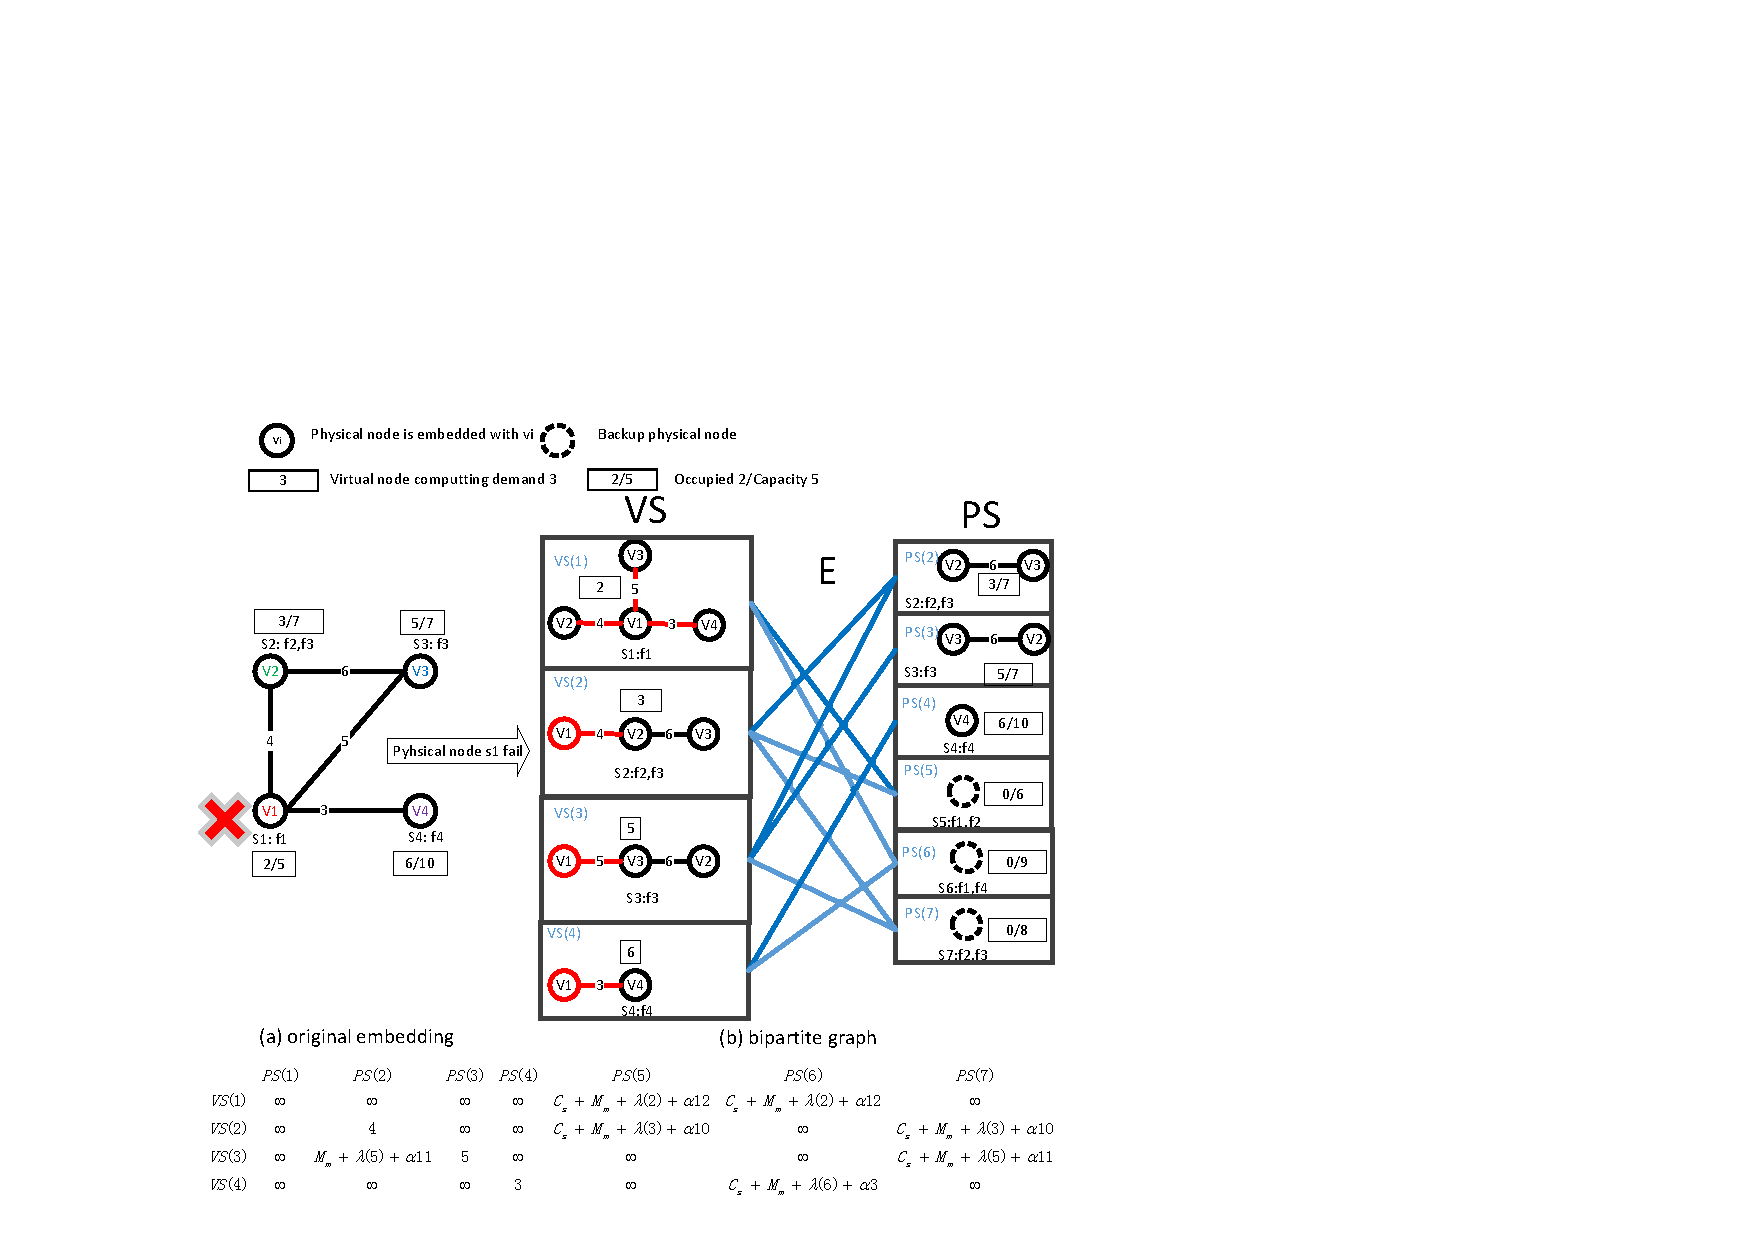
\includegraphics[width=2.5in]{Fig/StarRepresentation}\\
  \caption{The star representation of the former embedded virtual graph ($STAR_L$) and residual task graph after failure of node $v_1$ ($STAR_R$);}\label{fig:StarRepresentation}
\end{figure}

we define $\lambda(star_x,star_y)$ according to graph edit distance\cite{sanfeliu1983distance}.In mathematics and computer science, graph edit distance (GED) is a measure of similarity (or dissimilarity) between two graphs.

In this way, both the former embedded virtual graph and the residual graph which is after specific virtual node failure could be represented as a multiset of star structures. With such a graph decomposition, an alignment matrix of these star structures could be constructed with the alignment cost definition above. Therefore, the proposed GAP could be transformed to a (multiple knapsack problem) which will be investigated in the following part. The alignment cost matrix when virtual network $v_1$ fail as show in Equation \ref{lab:Node1FaliureAlignmentMatrix}.
\begin{equation*}
\tiny{
\left[ {\begin{array}{*{20}{c}}
&C_{V_{2}}&C_{V_3}&C_{V_4}&C_{B_{1}}&C_{B_{2}}&C_{B_{3}}\\
{R_{V_1}}&\infty&\infty&\infty&\fbox{N+(2)+4+5+3}&${N+(2)+4+5+3}$&\infty\\
R_{V_2}&\fbox{4}&\infty&\infty&${N+(3)+4+6}$&\infty&${N+(3)+4+6}$\\
R_{V_3}&${M+(2)+5}$&\fbox{5}&\infty&\infty&\infty&${N+(5)+5+6}$\\
R_{V_4}&\infty&\infty&\fbox{3}&\infty&${N+(6)+3}$&\infty\\
\end{array}} \right]
}
\label{lab:Node1FaliureAlignmentMatrix}
\end{equation*}

To elaborate this approach, Figure \ref{fig:StarRepresentation} shows how the 4-node VN in Fig.\ref{fig:GraphDecomposition} be decomposed into a multiset four five star structures (shown as $STAR_L$ ), and each containing a primary task node (also called root node which is highlighted), its adjacent links and its neighboring nodes.

\subsection{Multiple Knapsack Problem}
Based on the discussion above, the computation problem of minimal graph alignment cost is equivalent to solving optimal multiple knapsack problem, which is one of the fundamental combinational optimization problems concerned. In our case, there are two sets of vertices corresponding to the two multisets of star structures of $STAR_L$ and $STAR_R$ , and the weight of the edge between star structures of $STAR_L$ and $STAR_R$ is the alignment cost between the corresponding two stars. Then, Dynamic Programming algorithm could be applied to solve the multiple knapsack problem in $O[(n+b)*n*\prod_{i=1}^{n+b}C^i]$ time. Space complexity is $n*\prod_{i=1}^{n+b}C^i$.


\subsubsection{Dynamic Programming Equation}
\label{lab:DynamicProgrammingEquation}
initial state: $dp[i][{W_1}][{W_2}] \ldots [{W_m}]=0$ is assigned as infinity $\infty$.

$dp[0][{W_1}][{W_2}] \ldots [{W_m}]=0$: when there is no any virtual node which is confirmed to  map to another node. the total cost of current state is zero.

$dp[i][{W_1}][{W_2}] \ldots [{W_m}] $: when  i nodes is succeeded to be mapped another nodes. The total cost of current state is minimal cost from optimal node location.

state transfer equation as shown in Equ.\ref{equ:statetransferequation}: when put i-th node into another node, in this situation, the current state is calculated from former i-1 nodes is succeeded to be mapped.

\begin{equation}
\tiny{
\label{equ:statetransferequation}
dp[i][{W_1}][{W_2}] \ldots [{W_m}] = \min \left\{ \begin{array}{l}
dp[i - 1][{W_1} - {w_i}][{W_2}] \ldots [{W_m}] + {v_i}\\
dp[i - 1][W][{W_2}_{} - {w_i}] \ldots [{W_m}] + {v_i}\\
dp[i - 1][W][{W_2}_{}] \ldots [{W_m} - {w_i}] + {v_i}
\end{array} \right\}
}
\end{equation}



\subsection{Algorithm procedure}

\begin{algorithm}
\caption{survivable embedded virtual network request algorithm}
\label{alg:SeVNAlg}
\begin{algorithmic}[1]
\REQUIRE $G_{VN}(V^V,E^V,S^V,L^V)$: virtual network's topological graph with specific services; $B(V,S)$ backup nodes with specific services. $G_{SN}(V^S,E^S,S^S,L^S)$: substrate network's topological topological graph with specific services.
\ENSURE generate SeVN and SeVN into SN.
\STATE embed VN $G_{VN}$ into SN $G_{SN}$.
\STATE abstract embedded virtual network eVN.
\STATE decompose eVN into star struture set $STAR$.
%\STATE AllMinimumCycle($G(V,E)$)
\FORALL{$star_i$ such that $star_i\in STAR$}
\STATE construct items based star struture set $STAR$.
\STATE construct knapsacks based embedded virtual network eVN.
\STATE construct alignment cost matrix based graph edit distance method
\STATE solve multiple knapsack problem through dynamic programing
\STATE boot new nodes and connect new link in eVN
\STATE embed new additional backup resource from eVN into substrate network $G_{SN}$
\ENDFOR
\RETURN $G_{SN}$
\end{algorithmic}
\end{algorithm}





